% Phase 2 working draft. Historical October artifacts remain unchanged.
\documentclass[11pt]{article}
\usepackage[utf8]{inputenc}
\usepackage[T1]{fontenc}
\usepackage{lmodern}
\usepackage[margin=1in]{geometry}
\usepackage{amsmath,amssymb,amsthm}
\usepackage{booktabs,array,longtable,graphicx,xcolor}
\usepackage[round]{natbib}
\usepackage[colorlinks=true,allcolors=blue!50!black]{hyperref}
\newtheorem{proposition}{Proposition}
\theoremstyle{definition}
\newtheorem{assumption}{Assumption}
\newcommand{\E}{\mathbb E}
\newcommand{\Prb}{\mathbb P}
\newcommand{\pos}[1]{\left(#1\right)^+}
\newcommand{\Vtag}{\textnormal{[V]}}
\newcommand{\Ctag}{\textnormal{[C]}}
\newcolumntype{P}[1]{>{\raggedright\arraybackslash}p{#1}}
\raggedbottom
\title{Required Reserves, Public-Support Eligibility,\\and Voluntary Buffers}
\author{Carlos G\'omez Puic\'an\thanks{Universidad del Pac\'ifico. AI \& Economic Modeling, Track B: thesis model. Repository: \url{https://github.com/carlosgomezp28/ai-project}. The proposed V5.1 thesis architecture is joint work with Fabi\'an M\'endez Su\'arez under Marco Ortiz. The direct-support restriction and course optimization closure are the individual contribution developed here.}}
\date{Working title and first paper-core draft: 3 November 2026}
\begin{document}
\maketitle
\begin{abstract}
\noindent How do required reserves and public-support eligibility affect voluntary buffers? A bank with fixed deposits chooses liquidity before a shock. Buffers reduce shortfalls but displace the earning asset that determines public eligibility. In a direct-support benchmark, linear assistance and deferral costs give a convex private problem, an exact constrained optimality characterization, and sufficient conditions for uniqueness. At a regular interior optimum, a higher average reserve burden weakly reduces buffers when reserve usability is at least the eligibility coefficient; otherwise the sign is ambiguous. Deterministic finite-uniform illustrations verify the formulas under constructed parameters, not estimates for Peruvian banks. The broader joint V5.1 architecture and its OTC extension remain provisional. Lean formalization is planned and has not yet been performed.
\end{abstract}

\section{Introduction}
A bank can insure itself against a liquidity need by holding reserves voluntarily. The protection has an opportunity cost: liquidity displaces earning assets. If public assistance is limited by those assets, the same portfolio adjustment also reduces the bank's access to support. The question in this paper is how required reserves and asset-linked public-support eligibility shape the optimal voluntary buffer when these two margins are accounted for together.

The analytical contribution is a private optimization closure within a proposed thesis framework. The bank chooses a buffer per unit of deposits before observing liquidity needs. Required reserves may be partly usable during the episode. After the shock, the analytical core permits eligible public assistance and costly deferral, with no interbank financing. This restriction makes the assistance decision explicit and separates the portfolio mechanism from unresolved search and matching choices. It does not permanently remove the interbank mechanism from the project.

Two results organize the argument. First, the private problem is convex and admits a minimizer, with exact lower-corner, interior, and upper-corner conditions. At an interior optimum the marginal cost of liquidity equals a weighted sum of two shortfall probabilities. The severe-shortfall term is multiplied by one minus the eligibility coefficient: another buffer unit reduces the liquidity need but also reduces the asset backing assistance. Neither universal interiority nor universal strict convexity is claimed.

Second, at a unique regular interior optimum, a higher average required-reserve burden has a weakly negative buffer response when usability is at least the eligibility coefficient. When usability is lower, the sign is generally ambiguous. The result holds with costs, equity, eligibility, usability, and the shock law fixed. It is a local conditional comparative static, not a statement about optimal reserve policy, welfare, or an equilibrium with interbank feedback.

The proposed V5.1 thesis architecture is joint work by Carlos G\'omez Puic\'an and Fabi\'an M\'endez Su\'arez, supervised by Marco Ortiz. Its model-decision memo, dated 28 October 2026, remains pending advisor validation on explicitly open architecture choices. Carlos's individual AI-course contribution is the direct-support restriction, explicit buffer optimization closure, analytical propositions and proofs, verification, simulations, and formalization effort. No sole authorship of the joint baseline is claimed. No Lean theorem has yet been proved for this paper.

The existing illustrations use finite aggregate states and conditional uniform shocks. They are deliberately constructed examples, not estimates for Peruvian banks. Baseline voluntary buffers are quantitatively large, approximately 30 and 49 percent of deposits. Their purpose is to expose the mechanism and check formulas, not to predict observed bank portfolios. Heterogeneous incidence means a difference in optimized expected private cost per deposit under a specified counterfactual. It is not a measure of public transfers or social losses.

\section{Joint V5.1 baseline and related literature}
\paragraph{Relationship to the joint proposal.}
The joint memo proposes one currency at a time, two types without automatic size labels, a historical-Base reserve rule, ex ante voluntary reserves, heterogeneous shock exposure, and individual public eligibility. Its wider interbank architecture is provisional. The present paper solves a restricted continuation problem in which assistance and deferral are the available responses to a shortfall. The linear penalty, explicit cost criterion, distributional regularity, and optimization characterization are maintained course assumptions rather than advisor-approved conclusions.

The October course milestone studied a different mechanism, \emph{Public Dollar Backing and Voluntary Bank Buffers}, within an older joint IE1 baseline. It used interbank coverage and pooled dollar-capacity schedules held fixed across backing scenarios. Its conditional backing result remains part of the historical proposal and topic deck. It is not reproduced as a current proposition: the direct-support core has individual eligibility rather than the old aggregate public-capacity parameter. The historical artifacts remain unchanged.

\paragraph{Liquidity management and interbank architecture.}
\citet{bianchi2022} develop a banking liquidity-management model with an OTC interbank market, reserve settlement of deposit transfers, and a lending--liquidity trade-off. Their published article is in \emph{Econometrica} 90(1), pp.~391--454. This paper shares the portfolio trade-off but does not reproduce that interbank equilibrium or its monetary-policy applications. Its earning asset is residual, deposits are fixed, and the analytical continuation problem is direct public support. The individual contribution claimed here is an explicit eligibility-aware buffer closure inside the specified joint framework, not the discovery of precautionary reserves or OTC banking frictions.

\paragraph{Public support and private incentives.}
The October literature remains relevant at the mechanism level. \citet{ratnovski2009} studies liquidity choices distorted by expected lender-of-last-resort support. \citet{farhi2012} study the interaction of public intervention and strategic private balance-sheet choices. Here public prices and eligibility coefficients are given, and no strategic complementarity or bailout-policy equilibrium is derived. \citet{freixas2011} study liquidity uncertainty, interbank allocation, and central-bank policy; \citet{rochet2004} provide a coordination-based rationale for assistance when private markets fail to supply liquidity. Those allocation and coordination mechanisms lie outside the solved restriction.

These are bounded comparisons, not a literature-wide novelty claim. Bianchi--Bigio's published article and publisher metadata were checked; the other four references are the published articles used at the October milestone. Detailed proposition/page comparisons across appendices, working-paper versions, and citing papers remain incomplete. No assertion that those sources lack this exact closure is needed for the results below. The journal versions, rather than unverified new preprints, are cited.

\paragraph{Institutional motivation.}
The foreign-currency general regime in \citet[arts.~7--8, pp.~3--4]{bcrp2026} distinguishes an entity's historical Base and Base rate from the 35 percent rate above Base. Article~8 also caps the general-regime average rate. The model below stylizes the Base distinction; it omits that cap, deductions, special cases, and additional requirements. The circular's monthly averaging and reserve composition do not identify intraperiod usability. Thus neither $\phi$ nor the modeled eligibility rule is inferred from it. Institutional motivation is not a complete empirical description of Peru.

\section{Model}
All quantities below are per deposit unless an amount is explicitly identified. The tags \Vtag\ and \Ctag\ distinguish proposed joint V5.1 architecture from additional course restrictions or closure. Neither tag denotes advisor approval. The two banks solve separate private problems in the analytical core; the model does not jointly clear an interbank market.

\subsection{Environment, timing, and information}
\begin{assumption}[Environment and reserve treatment \Vtag]\label{ass:environment}
One currency is studied at a time. There are two types $k\in\{1,2\}$, with exogenous deposits $d_k>0$, historical Base $B_k\ge0$, Base rate $\tau_k^B\in[0,1]$, and marginal rate $\rho_m\in[0,1]$. During the episode these inputs are predetermined. The stylized required-reserve amount and average burden are
\begin{equation}\label{eq:reserve}
R_k(d_k)=\tau_k^B\min\{d_k,B_k\}+\rho_m(d_k-B_k)^+,
\qquad r_k=R_k(d_k)/d_k.
\end{equation}
Types are not assigned permanent borrower/lender or large/small roles.
\end{assumption}

The episode has three accounting dates. At $t_0$, the bank chooses its buffer knowing the parameters and shock law. At $t_1$, the liquidity need is realized and the bank chooses assistance and deferral. At $t_2$, obligations remain payable. These dates do not specify a full dynamic maturity, deposit-supply, or default model. Realized shocks are not known at portfolio choice.

\subsection{Required reserves and balance sheet}
\begin{assumption}[Feasible portfolio \Vtag\ + \Ctag]\label{ass:balance}
Equity per deposit is common, $E_k/d_k=\epsilon_E\ge0$, and
\begin{equation}\label{eq:balance}
b_k+R_k(d_k)+u_kd_k=d_k+E_k.
\end{equation}
Maintain $b_k\ge0$, $u_k\ge0$, and
\begin{equation}\label{eq:feasible}
U_k:=1+\epsilon_E-r_k>0,\qquad
0\le u_k\le U_k,\qquad b_k/d_k=U_k-u_k.
\end{equation}
The accounting identity is proposed architecture; the explicit nonnegative-asset restriction and feasible-set closure are maintained in the course benchmark.
\end{assumption}

When $d_k>B_k$, equation~\eqref{eq:reserve} gives
\begin{equation}\label{eq:average}
r_k=\rho_m-\frac{B_k}{d_k}(\rho_m-\tau_k^B).
\end{equation}
When $B_k\ge d_k$, $r_k=\tau_k^B$. At fixed deposits and $B_k<d_k$, the derivatives are $(\tau_k^B-\rho_m)/d_k$ with respect to Base and $B_k/d_k$ with respect to Base rate. Larger Base lowers burden only if the Base rate is below the marginal rate. At $B_k=d_k$ the branches join, but a Base derivative may change. Because deposits are fixed, these relations do not establish a distortion of a deposit-choice margin.

\subsection{Liquidity need and usable reserves}
\begin{assumption}[Liquidity convention and eligibility \Vtag\ + \Ctag]\label{ass:liquidity}
The liquidity need is $e_k=\beta_kA+\varepsilon_k$, where $A$ is the aggregate state and $\varepsilon_k$ is idiosyncratic. Larger positive realizations worsen liquidity; $e_k$ need not always be positive. Usable liquidity and the assistance limit are
\begin{equation}\label{eq:liquidity}
\widetilde u_k=u_k+\phi r_k,\qquad H_k(u_k)=\chi(U_k-u_k),
\end{equation}
with fixed $0\le\phi\le1$ and $0\le\chi<1$. Usability $\phi$ and asset-linked eligibility are provisional modeling interpretations. The restriction $\chi<1$ is additional to the joint memo and matches the implemented course domain.
\end{assumption}

Here $\phi$ means reserve usability, not the October public-coverage fraction. Eligibility is not a statement that all earning assets constitute usable collateral. A buffer is a ratio: raising $u_k$ by one raises voluntary reserves by $d_k$ in amounts. With deposits fixed, that change lowers $b_k/d_k$ by one and $H_k$ by $\chi$.

\subsection{Direct public support and deferral}
\begin{assumption}[Direct-support restriction \Vtag\ + \Ctag]\label{ass:direct}
There is no interbank financing in the analytical core. Gross shortfall is
\begin{equation}\label{eq:shortfall}
q_k=(e_k-u_k-\phi r_k)^+.
\end{equation}
Given $q_k,H_k$, the bank chooses $(W_k,v_k)$ satisfying
\begin{equation}\label{eq:continuation-constraints}
W_k+v_k=q_k,\qquad 0\le W_k\le\min\{q_k,H_k\},\qquad v_k\ge0.
\end{equation}
This is a restriction of the proposed wider architecture, not a decision to eliminate the OTC extension permanently.
\end{assumption}

\begin{assumption}[Incremental private costs \Ctag]\label{ass:cost}
Continuation cost is $pW_k+\Gamma(v_k)$ with $\Gamma(v)=gv$, where $g>p\ge0$. Reserve opportunity cost is $c(r_k+u_k)$ with $c>0$. These coefficients are fixed common primitives within each pure experiment, expressed in comparable episode units. Assistance and deferred principal remain liabilities; the criterion measures incremental private liquidity-management costs.
\end{assumption}

The criterion is maintained rather than derived from a complete terminal net-worth model. It does not say that deferred principal disappears or that public assistance is a gift. Neither $p$ nor $g$ is identified as an observed annual rate. Treating required and voluntary reserves as having a common net carrying cost is a deliberate simplification. A different remuneration or repayment specification would require a new objective, not a reinterpretation of these results.

\subsection{Ex ante voluntary-buffer problem}
\begin{assumption}[Analytical shock law \Ctag]\label{ass:law}
The aggregate state has a finite distribution. The induced liquidity need $e_k$ has $\E|e_k|<\infty$ and a continuous CDF $F_k$. The law is independent of the bank's buffer. Conditional shock laws need not be uniform for the general analytical characterization.
\end{assumption}

The bank minimizes reserve carrying cost plus optimized expected continuation cost over~\eqref{eq:feasible}. Proposition~\ref{prop:buffer} derives its explicit objective. No cross-bank idiosyncratic independence assumption is required for these separate problems. The aggregate-state decomposition gives economic meaning to exposure; the proof uses the induced marginal distribution of $e_k$.

\begin{assumption}[Finite-uniform implementation \Ctag]\label{ass:uniform}
For closed forms, simulation, and the planned finite algebraic formalization, $\Prb(A=A_j)=w_j$, with $w_j\ge0$ and $\sum_jw_j=1$, and
\begin{equation}\label{eq:uniform}
\varepsilon_k\mid A=A_j\sim U[-\sigma_{kj},\sigma_{kj}],\qquad \sigma_{kj}>0.
\end{equation}
This specialization implies Assumption~\ref{ass:law}; it is not required by the general Proposition~\ref{prop:buffer}.
\end{assumption}

\begin{assumption}[Local regularity and reserve variation \Ctag]\label{ass:regular}
At a point $(u_0,r_0)$, the CDF has a continuous nonnegative density in open neighborhoods of the two thresholds defined below. For the reserve response, $r_0$ is interior to an admissible burden interval, $0<u_0<U(r_0)$, the interior FOC holds, and $J_{uu}(u_0,r_0)>0$. Vary $r$ locally with $U(r)=1+\epsilon_E-r>0$, holding $c,p,g,\phi,\chi,\epsilon_E,\beta$ and the shock law fixed. In the finite-uniform implementation, exclude positive-weight support endpoints at either threshold.
\end{assumption}

This local density condition is stronger than atomlessness. It is needed for a regular second-derivative and implicit-function argument, not for existence or the first-order constrained characterization. Reserve variation means variation of average burden. Its implementation through Base or a reserve rate must be stated separately.

\section{Analytical results}
\subsection{Proposition 1: eligibility-aware optimal-buffer characterization}
Suppress the type index. Write $\overline F(t)=1-F(t)=\Prb(e>t)$ and define
\begin{equation}\label{eq:thresholds}
t_1(u)=u+\phi r,\qquad
t_2(u)=\phi r+\chi U+(1-\chi)u=t_1(u)+H(u).
\end{equation}
Thus $t_2\ge t_1$ on the feasible interval. The first threshold identifies any gross shortfall; the second identifies deferral after eligible assistance.

\begin{proposition}[Eligibility-aware optimal-buffer characterization]\label{prop:buffer}
Under Assumptions~\ref{ass:environment}--\ref{ass:law}, the continuation problem has the unique solution
\begin{equation}\label{eq:recourse}
W^*=\min\{q,H\},\qquad v^*=(q-H)^+.
\end{equation}
The ex ante problem is $\min_{u\in[0,U]}J(u)$, where
\begin{equation}\label{eq:objective}
\begin{split}
J(u)={}&c(r+u)+p\E\pos{e-t_1(u)}\\
&+(g-p)\E\pos{e-t_2(u)}.
\end{split}
\end{equation}
It is finite, continuous, and convex, and has a nonempty compact minimizer set $M$. Its first derivative is continuous, with feasible one-sided endpoint values, and
\begin{equation}\label{eq:foc}
J'(u)=c-p\overline F(t_1(u))-(g-p)(1-\chi)\overline F(t_2(u)).
\end{equation}
The exact constrained optimality conditions are
\begin{equation}\label{eq:corners}
\begin{aligned}
0\in M&\ \Longleftrightarrow\ J'(0)\ge0,\\
u\in M\quad(0<u<U)&\ \Longleftrightarrow\ J'(u)=0,\\
U\in M&\ \Longleftrightarrow\ J'(U)\le0.
\end{aligned}
\end{equation}
Endpoint membership does not assert that the endpoint is the only minimizer. Where the local density condition in Assumption~\ref{ass:regular} holds,
\begin{equation}\label{eq:curvature}
J''(u)=pf(t_1(u))+(g-p)(1-\chi)^2f(t_2(u))\ge0.
\end{equation}
An interior stationary point with strictly positive local curvature is the unique global minimizer. The strict inequalities $J'(0)>0$ or $J'(U)<0$ also give uniqueness of the respective endpoint. Otherwise uniqueness is not asserted; nonunique minima can occur. Uniformity in Assumption~\ref{ass:uniform} is unnecessary for these general claims.
\end{proposition}

\begin{proof}
\emph{Continuation and positive-part reduction.}
For feasible $q,H\ge0$, substitute $v=q-W$ into the continuation cost:
\[
pW+g(q-W)=gq-(g-p)W.
\]
Since $g-p>0$, this cost is strictly decreasing over the nonempty feasible interval $[0,\min(q,H)]$. Its unique minimizing assistance is its upper endpoint. The associated deferral is $q-\min(q,H)=(q-H)^+$, proving~\eqref{eq:recourse}, including $q=0$ or $H=0$.

For $H\ge0$, $(a^+-H)^+=(a-H)^+$. If $a\le0$, both sides are zero; if $a>0$, replace $a^+$ by $a$. Applying this identity with $a=e-u-\phi r$ gives
\begin{align*}
v^*&=\pos{e-u-\phi r-\chi(U-u)}\\
&=\pos{e-\phi r-\chi U-(1-\chi)u}=\pos{e-t_2(u)}.
\end{align*}
Also $q=\pos{e-t_1(u)}$ and $W=q-v$. Therefore
\[
pW+gv=p(q-v)+gv=pq+(g-p)v.
\]
Adding carrying cost and taking expectations proves~\eqref{eq:objective}. The reduction relies on $H\ge0$, which follows from feasibility.

\emph{Finiteness, continuity, convexity, and existence.}
Define $L(t)=\E\pos{e-t}$. The bound $(e-t)^+\le|e|+|t|$ ensures finiteness. Moreover,
\[
|(e-t)^+-(e-s)^+|\le|t-s|,
\]
so $L$ is Lipschitz and hence continuous. For each realization of $e$, the positive part of an affine function of $u$ is convex. Expectations and nonnegative weighted sums preserve convexity. Since $p\ge0$, $g-p>0$, and carrying cost is affine, $J$ is convex and continuous. The interval $[0,U]$ is nonempty and compact. The extreme-value theorem gives existence; continuity makes the minimizer set closed, and convexity makes it convex. It is consequently a nonempty compact interval, possibly a singleton.

\emph{First and second derivatives.}
For $h\ne0$, the absolute difference quotient of $(e-t)^+$ with respect to $t$ is at most one. Its limit is $-\mathbf1_{\{e>t\}}$ unless $e=t$. Atomlessness gives $\Prb(e=t)=0$. Dominated convergence therefore yields
\[
L'(t)=-\Prb(e>t)=-\overline F(t).
\]
The CDF is continuous, so this derivative is continuous. As $t_{1,u}=1$ and $t_{2,u}=1-\chi$, the chain rule gives~\eqref{eq:foc}. At feasible endpoints the same calculation gives the appropriate one-sided derivative. Where $F$ has the local continuous density specified in Assumption~\ref{ass:regular}, differentiating $\overline F(t_i)$ gives $-f(t_i)t_{i,u}$, which proves~\eqref{eq:curvature}. No derivative of a density is required.

\emph{Constrained optimality.}
For differentiable convex $J$, a feasible point minimizes cost exactly when
\begin{equation}\label{eq:variational}
J'(u^*)(z-u^*)\ge0\qquad\text{for every }z\in[0,U].
\end{equation}
Sufficiency follows from the convex tangent inequality. Necessity follows by taking feasible directional difference quotients at a minimum. At zero all feasible directions are nonnegative, giving $J'(0)\ge0$. At $U$ they are nonpositive, giving $J'(U)\le0$. At an interior point both signs of direction are feasible, forcing $J'(u^*)=0$. Conversely each listed condition implies~\eqref{eq:variational}. These are exactly~\eqref{eq:corners}.

\emph{Sufficient uniqueness.}
If two distinct points minimize a convex function, convexity and minimality make it constant on their connecting segment. At an interior stationary point with locally continuous positive curvature, the derivative crosses zero strictly in a neighborhood, excluding such a segment. This proves unique global optimality. If $J'(0)>0$, the convex tangent inequality gives $J(z)>J(0)$ for every $z>0$; if $J'(U)<0$, it gives $J(z)>J(U)$ for every $z<U$. Non-strict endpoint inequalities alone do not decide uniqueness.
\end{proof}

The interior FOC is not a recommendation to discard constraints. The equivalent KKT system is
\begin{equation}\label{eq:kkt}
J'(u)-\mu_0+\mu_U=0,\quad
\mu_0,\mu_U\ge0,\quad
\mu_0u=0,\quad\mu_U(U-u)=0.
\end{equation}
At an interior solution both multipliers vanish. At zero, $\mu_0=J'(0)$; at $U$, $\mu_U=-J'(U)$. This also checks the signs in~\eqref{eq:corners}.

In economic terms the first probability in~\eqref{eq:foc} values gross-shortfall reduction at the public unit cost $p$. It does not mean every shortfall unit is publicly funded. The second probability adds the deferral premium where eligibility is exhausted. In a deferral realization, $q_u=-1$ but $H_u=-\chi$, so $v_u=-(1-\chi)$ and $W_u=-\chi$. Another buffer unit replaces $\chi$ units of assistance and $1-\chi$ units of deferral. The saving is $p\chi+g(1-\chi)$, which equals $p+(g-p)(1-\chi)$.

Positive shortfall probability does not ensure curvature: if both thresholds remain below the shock support, the expected shortfalls are affine and local curvature is zero. Flat minima are possible if marginal carrying cost exactly equals the constant marginal saving. In the existing verification fixture with $A=3$, uniform width $0.1$, $\chi=0$, $c=g=0.4$, and other baseline settings, all $u\in[0,0.9]$ minimize cost. This fixture checks nonuniqueness; it is not a representative banking scenario. Nor does a zero endpoint derivative necessarily imply nonuniqueness.

\subsection{Proposition 2: conditional reserve-burden response}
Write $U(r)=1+\epsilon_E-r$ and regard $J$ as a function of $(u,r)$. A change in $r$ is an average-burden comparison with the listed primitives fixed. It is not a claim about endogenous deposits or the full statutory rule.

\begin{proposition}[Local conditional reserve-burden response]\label{prop:reserve}
Under Assumptions~\ref{ass:environment}--\ref{ass:law} and~\ref{ass:regular}, let $(u_0,r_0)$ satisfy the regular interior conditions. There is a neighborhood of $r_0$ with a continuously differentiable, feasible interior optimal choice $u^*(r)$, unique there as a global minimizer, and
\begin{equation}\label{eq:response}
\frac{du^*}{dr}
=-\frac{p\phi f(t_1)+(g-p)(1-\chi)(\phi-\chi)f(t_2)}
{pf(t_1)+(g-p)(1-\chi)^2f(t_2)}.
\end{equation}
All thresholds are evaluated at $(u^*(r),r)$. If $\phi\ge\chi$, the response is weakly negative; strict negativity requires a strictly positive numerator. If $\phi<\chi$, the sign is generally ambiguous. The claim excludes corners, nonunique optima, zero curvature, and unsupported density-boundary evaluations. It does not extend to endogenous shock laws or OTC/search/matching/pricing feedback, and has no welfare or optimal-policy interpretation.
\end{proposition}

\begin{proof}
Let $G(u,r)=J_u(u,r)$. By Proposition~\ref{prop:buffer}, the interior optimality equation is
\begin{equation}\label{eq:G}
G(u^*(r),r)=c-p\overline F(t_1)-(g-p)(1-\chi)\overline F(t_2)=0.
\end{equation}
The relevant partial derivatives of the feasible bound and thresholds are
\begin{equation}\label{eq:threshold-partials}
U_r=-1,\quad t_{1,r}=\phi,\quad t_{2,r}=\phi-\chi,
\quad t_{1,u}=1,\quad t_{2,u}=1-\chi.
\end{equation}
In particular, $t_{2,r}=\phi+\chi U_r=\phi-\chi$; ignoring the balance-sheet dependence of eligibility would miss this term. Since the distribution is fixed and $\overline F'=-f$ locally,
\begin{align}
G_u&=pf(t_1)+(g-p)(1-\chi)^2f(t_2)=J_{uu}>0,
\label{eq:Gu}\\
G_r&=p\phi f(t_1)+(g-p)(1-\chi)(\phi-\chi)f(t_2).
\label{eq:Gr}
\end{align}
Although carrying cost includes $cr$, its derivative with respect to $u$ is the fixed constant $c$, so it contributes no additional term to $G_r$.

The continuous-density assumption makes $G$ continuously differentiable in an open neighborhood of the interior point. Equation~\eqref{eq:Gu} allows the implicit-function theorem to produce a continuously differentiable local root. Shrink the neighborhood so that $0<u^*(r)<U(r)$ and positive curvature persist. Convexity and the sufficient uniqueness part of Proposition~\ref{prop:buffer} then make this root the unique global minimizer locally in $r$.

Differentiate~\eqref{eq:G} along the root:
\[
0=G_u\frac{du^*}{dr}+G_r.
\]
Division by $G_u>0$ gives~\eqref{eq:response}. If $\phi\ge\chi$, both terms in~\eqref{eq:Gr} are nonnegative, establishing the weak sign and its strictness qualification. If $\phi<\chi$, the numerator instead is
\[
\underbrace{p\phi f(t_1)}_{\ge0}
-\underbrace{(g-p)(1-\chi)(\chi-\phi)f(t_2)}_{\ge0}.
\]
The assumptions impose no universal ordering between these quantities. A positive first term with $f(t_2)=0$ gives a negative response; a positive second term with a zero first term gives a positive response. Their equality gives zero. These density configurations are compatible with the maintained shock class.
\end{proof}

Usable required reserves substitute for voluntary liquidity through the first threshold. They also displace earning assets and hence reduce eligibility. The severe-shortfall threshold rises with burden only if usability exceeds that eligibility displacement. At $\phi=\chi$ the second channel cancels, but the first can still give a strictly negative response when $p\phi f(t_1)>0$.

The statement is local for substantive reasons. A larger change can move the optimum to a constraint or change the active support regions. For uniform mixtures, $J$ is globally $C^1$ but generally not globally $C^2$. At a support knot the theorem is not applied; a separate one-sided or case analysis would be necessary. The result also changes if prices, eligibility coefficients, usability, equity, or the shock law move with $r$. A Base comparison must additionally use the relevant branch of~\eqref{eq:reserve}; the kink at $B=d$ is not a regular two-sided Base derivative.

\section[Numerical illustrations and heterogeneous private-cost incidence]{Numerical illustrations and heterogeneous\\private-cost incidence}
\subsection*{Constructed parameters and reproducibility}
Only existing Phase~1 outputs are used. The code checkpoint is \texttt{7406387}; it is not a paper-formalization checkpoint. Table~\ref{tab:parameters} lists all baseline economic inputs. Expectations use exact uniform positive-part formulas and deterministic finite-state sums. Independent midpoint integration and objective-only grid comparisons check these calculations. There is no primary Monte Carlo calculation.

\begin{table}[htbp]
\centering\small
\caption{Illustrative constructed baseline parameters, not estimates for Peruvian banks. Symbols and architecture do not imply advisor approval.}\label{tab:parameters}
\begin{tabular}{@{}P{.18\linewidth}P{.18\linewidth}P{.58\linewidth}@{}}
\toprule Input & Value & Interpretation and comparison\\\midrule
$c$ & $0.035$ & Common opportunity cost of required and voluntary reserves\\
$p,g$ & $0.04,0.40$ & Public funding cost and linear deferral penalty\\
$\phi,\chi$ & $0.50,0.20$ & Common usability and eligibility coefficients\\
$\epsilon_E$ & $0.10$ & Common equity per deposit\\
$d_k,B_k$ & $1.00,0.60$ & Fixed deposits and historical Base\\
$\tau_k^B,\rho_m$ & $0.10,0.35$ & Common baseline reserve rates\\
$\beta_1,\beta_2$ & $1.00,1.35$ & Exposure difference in the baseline cost figure\\
$A_j$ & $0,0.45$ & Normal and adverse aggregate states\\
$w_j$ & $0.70,0.30$ & Corresponding state probabilities\\
$\sigma_{kj}$ & $0.20$ & Conditional uniform support half-width in every state\\
\bottomrule
\end{tabular}
\end{table}

The coefficients are in comparable episode units, not estimated annual rates. The large deferral premium $g-p=0.36$ makes severe shortfalls important. A larger $\beta$ raises adverse-state needs and the unconditional mean, so the exposure comparison is not a mean-preserving spread. No claim of robustness to every cost, shock, or equity choice is made.

\subsection*{Baseline buffers and the private trade-off}
Table~\ref{tab:outcomes} and Figure~\ref{fig:cost} show unique interior optima for the two baseline exposure types. Normal-state needs are fully absorbed at both optima. More exposed Type~2 chooses more liquidity, reduces its earning asset, and faces a smaller eligibility limit. It consequently uses less expected public assistance even though exposure is higher; expected deferral is slightly higher. Funding usage cannot be inferred from exposure alone without accounting for the endogenous portfolio.

\begin{table}[htbp]
\centering\small
\caption{Baseline outcomes under illustrative constructed parameters, not estimates for Peruvian banks. All quantities are per deposit. Source: existing \texttt{buffer\_type\_optima.csv}.}\label{tab:outcomes}
\begin{tabular}{@{}lrr@{}}
\toprule Outcome & Type 1 & Type 2\\\midrule
Required-reserve burden $r_k$ & 0.200000 & 0.200000\\
Feasible upper bound $U_k$ & 0.900000 & 0.900000\\
Voluntary buffer $u_k^*$ & 0.302860 & 0.493910\\
Earning asset $b_k/d_k$ & 0.597140 & 0.406090\\
Expected assistance $\E W_k$ & 0.016788 & 0.010537\\
Expected deferral $\E v_k$ & 0.006116 & 0.006571\\
Expected private cost $J_k^*$ & 0.020718 & 0.027337\\
Classification & Unique interior & Unique interior\\
\bottomrule
\end{tabular}
\end{table}

These are quantitatively large voluntary buffers: about 30 and 49 percent of deposits. Including required reserves, total reserves are about 50 and 69 percent. This feature must remain visible; the constructed shock magnitudes and costs were not selected to match observed banks. The baseline private-cost difference is $0.006618506$ per deposit. Reserve carrying costs account for most of that difference, rather than higher assistance usage.

\begin{figure}[htbp]
\centering
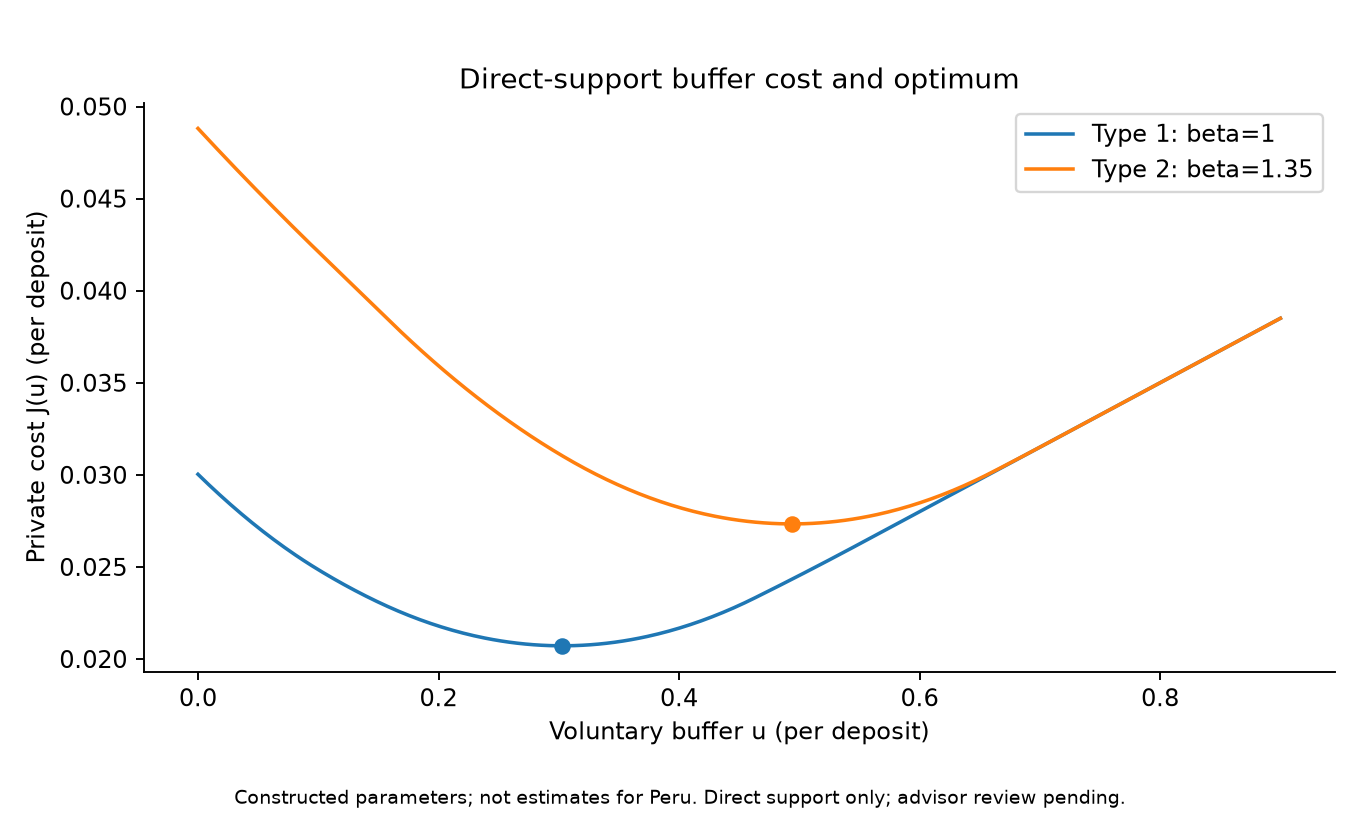
\includegraphics[width=.86\linewidth]{../code/figures/buffer_cost.png}
\caption{Private cost against the chosen buffer for the two exposure types; dots identify optima. Illustrative constructed parameters, not estimates for Peruvian banks. This illustrates Proposition~\ref{prop:buffer}, not universal interiority. Above $u=0.7075$ both types have no shortfall and their costs coincide. The vertical axis is truncated.}\label{fig:cost}
\end{figure}

\subsection*{Usability and the reserve response}
Figure~\ref{fig:usability} varies $r$ from $0.04$ to $0.44$ for Type~1 with $\chi=0.2$, using $\phi=0.6,0.2,0$. The helper realizes each burden through $B=d=1$ and $\tau^B=r$; this is an abstract burden path, not a sweep of the marginal rate. Other primitives and the shock law stay fixed. At $r=0.2$, the respective buffers are $0.278600$, $0.375641$, and $0.424162$, with local slopes $-0.514793$, $-0.029586$, and $+0.213018$.

Every saved point in these three panels is interior and remains in the same support configuration, producing straight lines. The equality case $\phi=\chi$ is not flat because the ordinary-shortfall channel remains. The positive response at $\phi=0$ illustrates eligibility displacement without immediate usable-reserve protection. It does not prove a positive response for every $\phi<\chi$ case. The three panels share a vertical scale, but their levels depend on the constructed parameter choices.

\begin{figure}[htbp]
\centering
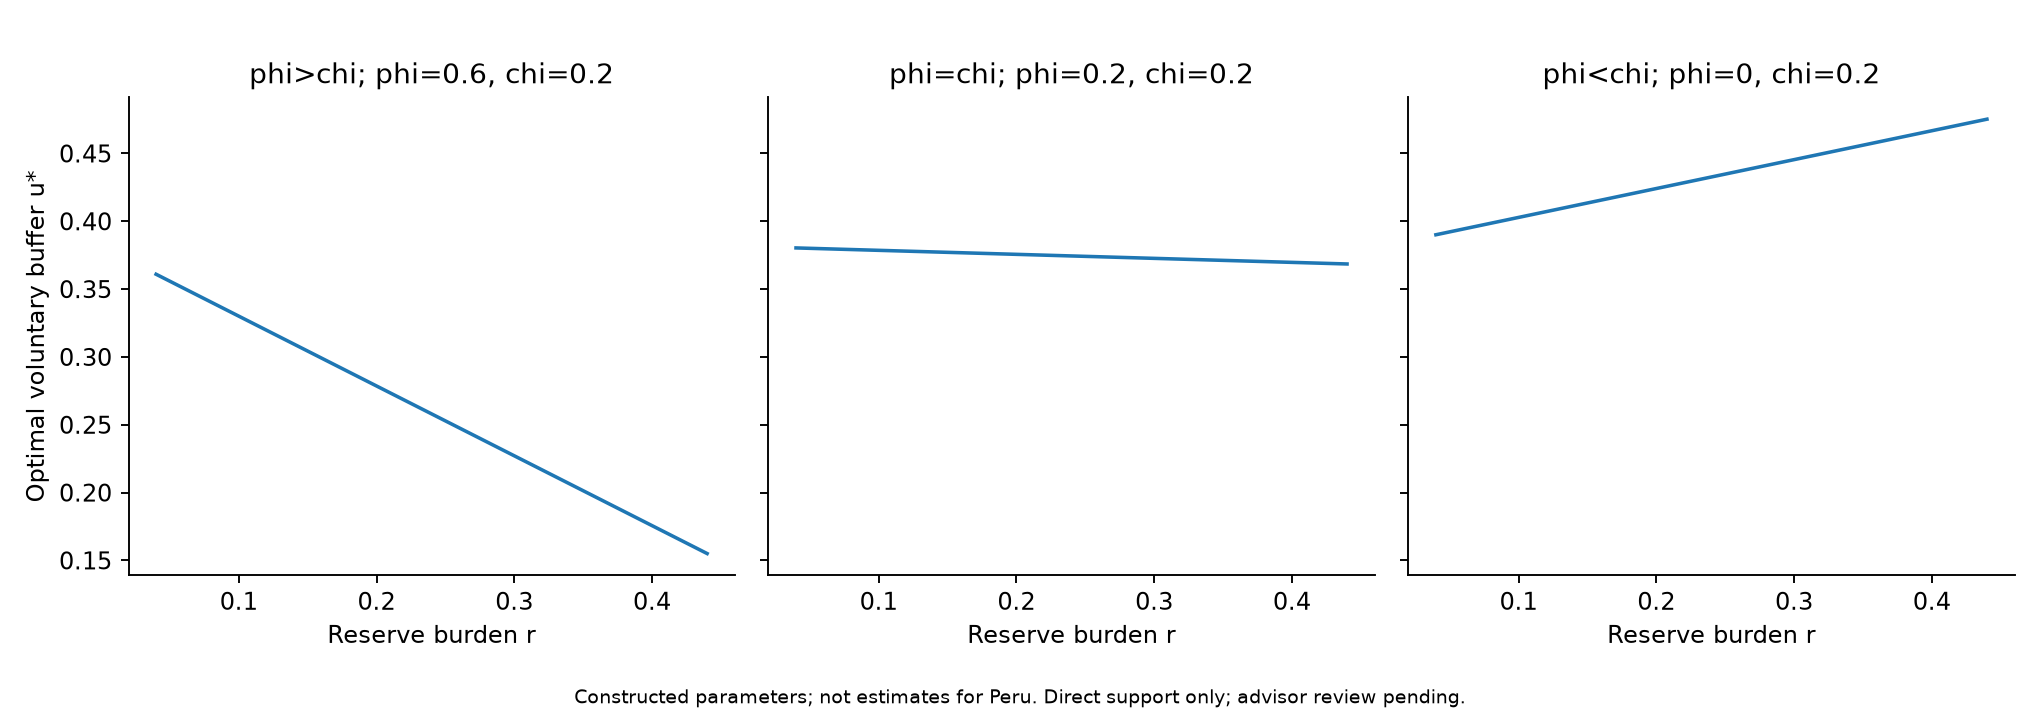
\includegraphics[width=\linewidth]{../code/figures/buffer_reserve_usability.png}
\caption{Optimal buffer against average reserve burden for three fixed usability values. Illustrative constructed parameters, not estimates for Peruvian banks. The figure illustrates the conditional sign in Proposition~\ref{prop:reserve}; it is neither an estimate of reserve-policy effects nor an equilibrium result. All plotted solutions are unique and interior.}\label{fig:usability}
\end{figure}

\subsection*{Regulatory counterfactuals and private-cost incidence}
Figure~\ref{fig:regulation} isolates regulatory treatment. Both types now have $\beta=1$; Type~1 retains $B=0.6$, $\tau^B=0.1$. Type~2 varies only Base in one experiment and only Base rate in the other, with deposits fixed. The label Type~2 therefore identifies a different isolated counterfactual from Figure~\ref{fig:cost}; it is not a permanently calibrated bank.

Raising Base from $0.1$ to $1$, with $\tau^B=0.1<\rho_m=0.35$, lowers burden from $0.325$ to $0.1$. The buffer rises from $0.253674$ to $0.342209$ and private cost falls from $0.023340$ to $0.018625$. Further Base increases to $1.2$ do nothing because all deposits are below Base. That flat segment is a reserve-rule feature, not an indifferent buffer choice or a buffer corner.

Raising Base rate from $0.02$ to $0.40$ at $B=0.6$ instead increases burden from $0.152$ to $0.38$. Buffers fall from $0.321748$ to $0.232032$, while earning assets fall from $0.626252$ to $0.487968$. Expected assistance falls from $0.017813$ to $0.013115$, expected deferral rises from $0.006049$ to $0.006374$, and private cost rises from $0.019713$ to $0.024495$. Lower voluntary buffers do not fully offset the higher required reserves. Reduced eligibility can worsen severe remaining needs even while usable reserves reduce gross shortfall.

\begin{figure}[htbp]
\centering
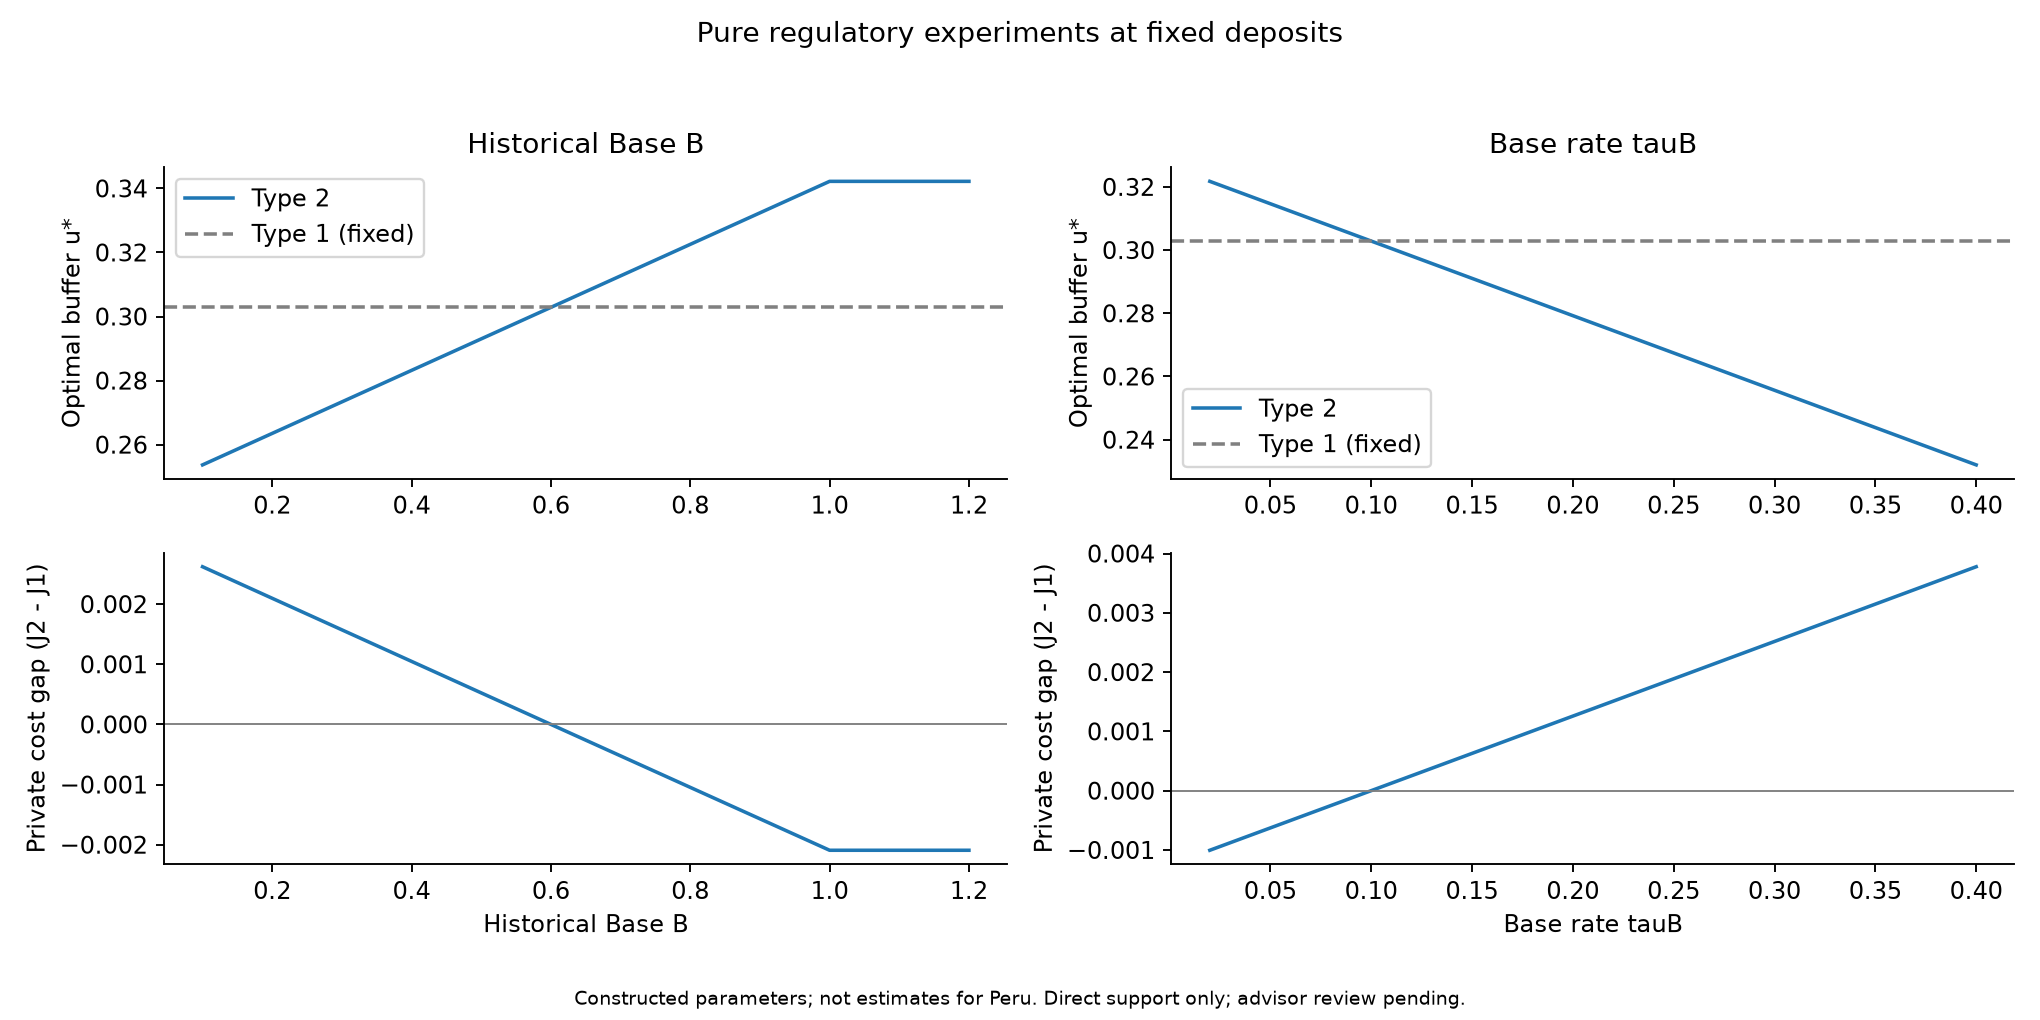
\includegraphics[width=\linewidth]{../code/figures/buffer_regulation.png}
\caption{Pure Base and Base-rate comparisons at fixed deposits. Upper panels show buffers; lower panels show $J_2^*-J_1^*$. Illustrative constructed parameters, not estimates for Peruvian banks or a legally validated policy range. Panel scales differ. The Base plateau follows the reserve rule. The figure concerns private-cost incidence, not welfare, subsidies, or fiscal cost.}\label{fig:regulation}
\end{figure}

Define heterogeneous private-cost incidence precisely as
\begin{equation}\label{eq:incidence}
\Delta J=\min_{[0,U_2]}J_2-\min_{[0,U_1]}J_1
\end{equation}
under a stated pair of counterfactuals. In the Base experiment this gap ranges from $+0.002622$ to $-0.002093$; in the Base-rate experiment it ranges from $-0.001005$ to $+0.003777$. Zero crossings identify equality with the fixed reference type, not a transfer between banks. A reserve-induced change in an exposure gap would require comparing that gap across reserve regimes; the single baseline exposure gap does not identify it.

These differences are not subsidies, net transfers, welfare losses, fiscal costs, or empirical causal effects. There is no financing or loss-allocation rule for a public insurance pool and no social objective. The numerical reserve ranges also need not satisfy all omitted provisions of the actual circular. In particular, the low-rate and high-average-burden tails are mathematical stress comparisons, not recommended or asserted legal positions.

\section{Provisional OTC/interbank extension and limitations}
The broader joint V5.1 proposal includes a provisional OTC, uncollateralized interbank market with heterogeneous access and bilateral Nash pricing. Access is represented by a ticket $a_k=1-e^{-\lambda_k}$, which is not effective funding probability. The analytical core sets this module aside while the search participation rule, lender outside option, effective matching, loan quantities, and Nash bargaining object await advisor validation or explicit closure. The present propositions must not be attached to that unresolved extension.

A consistent extension would replace the direct-support continuation value with a value including both sides of each trade. Borrower gains must be compared with direct assistance and deferral, including failed search. Lender participation needs an outside option and incremental cost. Each realized loan must obey available surplus and borrower-need bounds, with equal monetary amounts lent and received under consistent population weights. Pricing cannot replace quantity conservation. Uncollateralized repayment assumptions also need to be stated before a negotiated payment is interpreted.

The public continuation cost derived here remains a useful outside option for that extension. However, a buffer would then also change borrower need, lender surplus, participation, matching, negotiated quantities, or prices. Those effects are absent from~\eqref{eq:foc} and~\eqref{eq:response}. There is no completed OTC simulation or equilibrium result in this draft. One currency at a time similarly avoids pretending that simultaneous currency markets are isolated without addressing conversion.

Further limitations are substantive. Deposits and the shock law are exogenous; the earning asset is residual rather than chosen through a full credit-demand problem. The reserve rule omits regulatory components. Usability is a provisional episode parameter, eligibility is reduced-form, and the linear deferral penalty limits the continuation problem's richness. Costs are private and incremental, not a full terminal solvency or welfare account. The large constructed buffers are not calibration evidence. No theorem of optimal reserve design, fiscal saving, redistribution, or empirical Peruvian incidence follows.

\section{Conclusion}
In the direct-support restriction of the proposed joint V5.1 architecture, voluntary liquidity reduces shortfalls but displaces assets supporting public eligibility. The resulting private problem admits a convex constrained characterization, with uniqueness only under additional sufficient conditions. The local reserve response is weakly negative when usability is at least the eligibility coefficient and otherwise has an ambiguous sign. Existing constructed illustrations show the trade-off and its private-cost consequences without establishing empirical magnitudes. The remaining tasks are handwritten reproduction, faithful formalization, verified detailed literature positioning, and eventual closure of the provisional interbank module with advisor feedback.
\label{end:body}
\clearpage
\bibliographystyle{plainnat}
\begingroup\raggedright
\bibliography{references}
\endgroup
\clearpage
\appendix

\section{Uniform shortfall formulas and the implementation bridge}\label{app:uniform}
This appendix specializes Assumption~\ref{ass:law} using Assumption~\ref{ass:uniform}. It does not impose uniform shocks on the general proposition. For $\varepsilon\sim U[-\sigma,\sigma]$, $\sigma>0$, define $\ell_\sigma(z)=\E[(\varepsilon-z)^+]$. If $z\le-\sigma$, the positive part equals $\varepsilon-z$ almost surely, whose expectation is $-z$. If $z\ge\sigma$, it is zero. For $-\sigma<z<\sigma$,
\begin{align*}
\ell_\sigma(z)
&=\frac1{2\sigma}\int_z^\sigma(\varepsilon-z)\,d\varepsilon
=\frac1{2\sigma}\left[\frac{\varepsilon^2}{2}-z\varepsilon\right]_z^\sigma\\
&=\frac{\sigma^2/2-z\sigma+z^2/2}{2\sigma}
=\frac{(\sigma-z)^2}{4\sigma}.
\end{align*}
Thus the exact functions are
\begin{equation}\label{eq:uniform-functions}
\ell_\sigma(z)=\begin{cases}-z&z\le-\sigma,\\(\sigma-z)^2/(4\sigma)&-\sigma<z<\sigma,\\0&z\ge\sigma,\end{cases}
\quad
\Pi_\sigma(z)=\begin{cases}1&z\le-\sigma,\\(\sigma-z)/(2\sigma)&-\sigma<z<\sigma,\\0&z\ge\sigma.\end{cases}
\end{equation}
Here $\Pi_\sigma(z)=\Prb(\varepsilon>z)$. At the lower support join the value is $\sigma$ and slope $-1$; at the upper join the value and slope are zero. Therefore $\ell_\sigma$ is globally $C^1$ with derivative $-\Pi_\sigma$, and convex because that derivative is nondecreasing. Its second derivative is $1/(2\sigma)$ strictly inside the support and zero strictly outside. Global $C^2$ smoothness is not asserted.

For the finite mixture, set $z_{ij}=t_i-\beta A_j$. Then
\begin{align}
L(t)&=\sum_jw_j\ell_{\sigma_j}(t-\beta A_j),&
\overline F(t)&=\sum_jw_j\Pi_{\sigma_j}(t-\beta A_j),\label{eq:mixture}\\
f(t)&=\sum_j\frac{w_j}{2\sigma_j}\mathbf1_{\{|t-\beta A_j|<\sigma_j\}}.
\label{eq:mixture-density}
\end{align}
The density formula is used away from positive-weight support endpoints. Substitute~\eqref{eq:mixture} into~\eqref{eq:objective} to obtain the explicit finite algebraic objective $\widehat J$. This is the planned Lean implementation. Formal verification of its arithmetic and calculus alone would not verify its probabilistic interpretation without the integral bridge just derived.

For the current feasible interval, support-region boundaries occur at $t_1-\beta A_j=\pm\sigma_j$ or $t_2-\beta A_j=\pm\sigma_j$. Their buffer locations are
\[
u=\beta A_j\pm\sigma_j-\phi r,
\qquad
u=\frac{\beta A_j\pm\sigma_j-\phi r-\chi U}{1-\chi}.
\]
Only locations in $[0,U]$ with positive state weight matter. Between successive boundaries the FOC is affine, so the implementation finds its roots and tests endpoints. A flat minimizing interval is reported as nonunique with both interval endpoints; its left endpoint is only a reporting convention.

\section{Existing exposure illustration and verification coverage}\label{app:verification}
\begin{figure}[htbp]
\centering
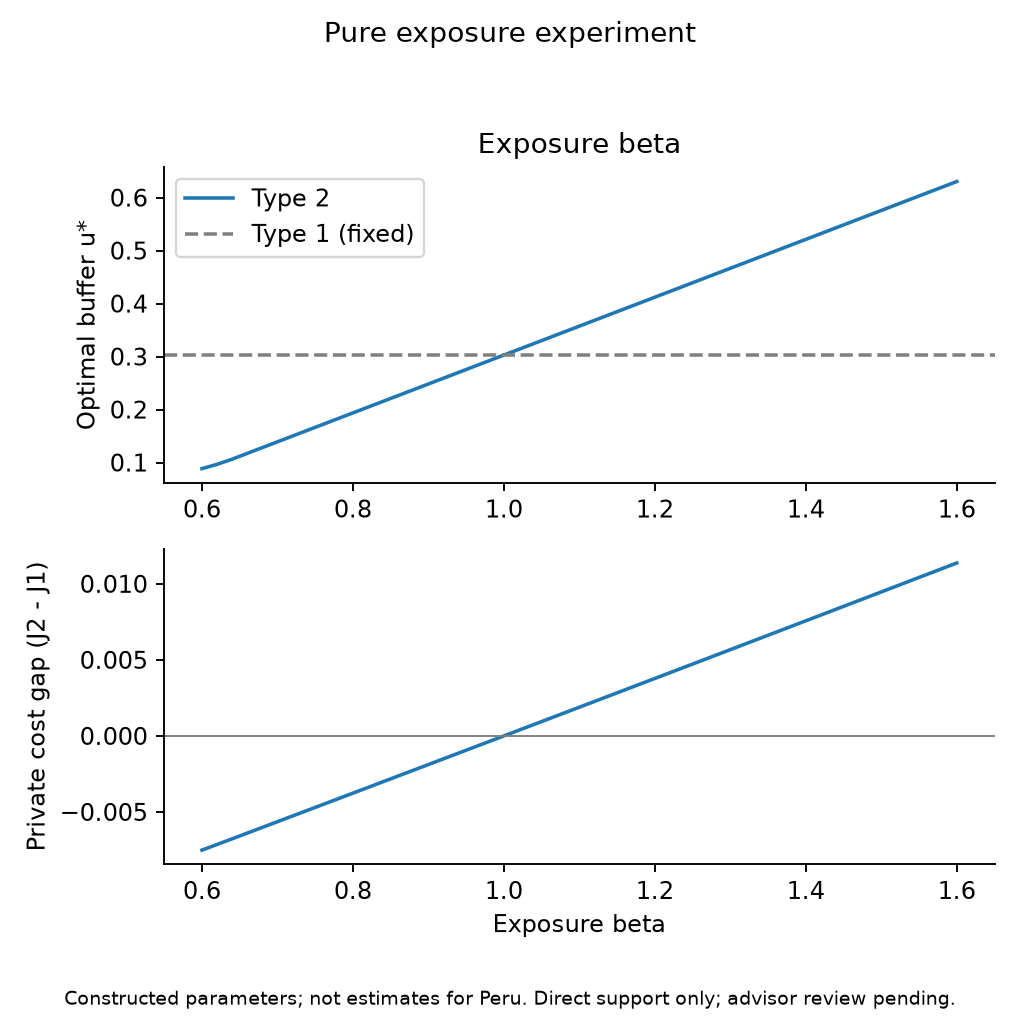
\includegraphics[width=.82\linewidth]{../code/figures/buffer_exposure.png}
\caption{Additional pure exposure illustration. Illustrative constructed parameters, not estimates for Peruvian banks. Type~2's $\beta$ varies with all other primitives fixed; Type~1 stays at $\beta=1$. The strict increase on this grid is not a general theorem about increases in risk.}\label{fig:exposure}
\end{figure}
The existing exposure grid has 51 values from $0.6$ to $1.6$, with buffers from $0.088490$ to $0.630375$. The private-cost gap ranges from $-0.007509$ to $+0.011370$ and is zero at identical primitives, $\beta=1$. A support transition between $0.62$ and $0.64$ changes the slope as normal-state shortfalls disappear. No plotted point is a corner or a nonunique solution.

The single entry point is \texttt{python code/verify.py}. Its historical section preserves 28 October checks and labels the old coverage and backing objects as historical. The new section has 38 course-core checks. The stored verification report records a maximum expected-positive-part integration error of $2.78\times10^{-11}$, a maximum objective-derivative finite-difference error of $7.51\times10^{-9}$, and a maximum reserve-response error of $5.97\times10^{-12}$ over 27 regular interior comparisons. Thirteen optimizer scenarios include both corners and nonunique minima. These are conditional checks, not formal proofs or calibration.

The saved economic outputs contain 537 experiment rows and 802 cost-curve rows. Every saved experiment optimum is unique and interior; corner and nonunique cases are separate verification fixtures. The closest saved optimum threshold to a support endpoint is approximately $0.003394$ away in the exposure experiment. No claim is made that every conceivable parameter value has been tested. The inherited \texttt{effort\_check.csv} and effort figure are template artifacts, not results of this banking model.

\section{Lean formalization status and correspondence}\label{app:lean}
\textbf{Current status: NOT YET FORMALIZED.} There is no Lean verification claim, generated paper folder, paper-formalization commit, or successful paper-scoped check to report. The code checkpoint \texttt{7406387} is not a substitute for any of these. The following table identifies obligations, not accomplished proofs.

\small
\begin{longtable}{@{}P{.20\linewidth}P{.42\linewidth}P{.32\linewidth}@{}}
\toprule Paper component & Planned Lean statement & Current status and boundary\\\midrule
\endhead
Proposition~\ref{prop:buffer}: continuation & Feasible unique minimizer $(\min(q,H),(q-H)^+)$ for $g>p$ & Open; real-order and min/max proof planned\\
Positive-part reduction & $(a^+-H)^+=(a-H)^+$ for $H\ge0$; optimized cost identity & Open; algebraic target, no probability claim\\
Appendix~\ref{app:uniform} calculus & Piecewise $\ell_\sigma$, joins, derivative $-\Pi_\sigma$, convexity & Open; integral interpretation is a separate bridge\\
Proposition~\ref{prop:buffer}: finite implementation & Derivative, existence, convexity, constraints, sufficient uniqueness for $\widehat J$ & Open; not automatically the general atomless proposition\\
Proposition~\ref{prop:reserve}: conditional identity & Chain-rule response and sign along a differentiable regular FOC branch & Open; branch existence requires an IFT proof or disclosed added hypothesis\\
Probabilistic and IFT bridges & Expected-shortfall derivative and local optimal-branch existence & Open; needed before claiming full general propositions are formalized\\
\bottomrule
\end{longtable}
\normalsize
The paper and Lean must use identical explicit finite-function definitions when that implementation is formalized. A successful polynomial calculation inside a support region is not a proof of global constrained optimality. Assuming an already differentiable FOC branch can be disclosed as an additional hypothesis; assuming the desired derivative formula would instead smuggle in the conclusion. Each numbered proposition will retain an explicit status until its precise statement is checked. The final appendix must report the actual pinned paper commit, declarations, files, added hypotheses, and paper-scoped check output.

\section{AI collaboration and human verification}\label{app:ai}
The AI-assisted workflow is declared. Raw October prompts and answers remain in \texttt{prompts.md}; final-stage interactions and Carlos's adjudications still need to be appended in a later authorized step. This draft distinguishes mathematical reasoning, executable checks, and unfinished formalization. The typed guide in \texttt{hand/} is not a substitute for handwritten work.

\begin{center}\small
\begin{tabular}{@{}P{.26\linewidth}P{.28\linewidth}P{.40\linewidth}@{}}
\toprule Claim or risk & Current assessment & Evidence and remaining work\\\midrule
Deficit derivative is minus a probability & Correct for normalized $L$; amount $S^-=dL$ has derivative $-d\pi^-$ & October provenance audit and normalization distinction; retain historical derivation\\
Positive deficit probability ensures curvature & False without a marginal support condition & Certain-deficit region is affine; new verification includes flat and corner fixtures\\
Old FOC transfers unchanged & Inapplicable when eligibility moves with buffers & Current proof derives $H_u=-\chi$ and the factor $1-\chi$; do not invent a past AI-rejection episode\\
New formulas establish empirical effects & Not supported & Constructed inputs, conditional checks, no estimates\\
Lean has verified the propositions & Not established & No formalization performed; Appendix~\ref{app:lean} records open targets\\
\bottomrule
\end{tabular}
\end{center}
The first row is the strongest documented correction candidate for the required defense discussion: units must be checked against the inherited source rather than trusting an unqualified derivative identity. Carlos must reproduce and record his own check and verdict; the draft does not assert an undocumented history of human rejection. Final-model handwritten derivations are still to be completed. No permission to publish private joint source documents is inferred from using them for local provenance checking.
\end{document}
